\documentclass[11pt]{article} 

\usepackage[utf8]{inputenc} 

\usepackage{graphicx}

\usepackage{geometry}
\geometry{a4paper} 


\title{Winterthur Yard: Projektidee}
\author{Maja Fritschi, Raphael Spörri, Florian Bosshard}
\date{} 
\begin{document}
\maketitle

\tableofcontents
\newpage

\section{Spielbeschreibung}
In diesem Projekt wird eine Schnitzeljagd ähnlich dem Spiel Scotland Yard, durch die Winterthurer Altstadt entwickelt. Daher auch die Projektbezeichnung Winterthur Yard. 

Ziel des Spiels ist es, MisterX zu fangen, der sich an verschiedenen Punkten in der Altstadt versteckt. Hat man MisterX gefangen, verrät er einem ein Geheimnis, beispielsweise die Koordinaten eines Geocaches \footnote{Versteck des Spiels Geocaching, siehe http://www.geocaching.com}. 

MisterX wird dabei dargestellt durch einen Computerspieler, der sich automatisiert von Punkt zu Punkt bewegt. Der Spieler geht durch die Stadt und versucht MisterX zu finden. Mittels Geolocation gibt er an den einzelnen Knoten seinen Standort bekannt. Wenn er am gleichen Ort ist wie MisterX, so hat er das Spiel gewonnen. Ansonsten sieht er, wo sich MisterX als letztes befunden hatte. Daneben wird ihm auch angezeigt, wo sich andere Spieler in diesem Moment gerade befinden. 

In der Applikation kann die Funktion "MisterX fangen" aufgerufen werden sobald man physisch an einem der definierten Knoten ist. Ist MisterX an diesem Knoten, so hat man das Spiel gewonnen. Ansonsten sieht man, wo sich MisterX als letztes befunden hatte. Zudem sieht man, wo andere Mitspieler sich befinden. So ist es möglich koordiniert miteinander vorzugehen. 

MisterX wechselt seinen Standort in einem definierten Zeitintervall und bewegt sich immer nur den Graphen zwischen den einzelnen Knoten entlang. Er gibt jeweils nur den Punkt an, an dem er als letztes war, nicht wo er sich aktuell befindet. 

\section{Ziele}
Für die Spielenden:
\begin{itemize}
\item Schöne Stellen in der Winterthurer Altstadt besuchen
\item Funktionalität des eigenen Mobiltelefons kennen lernen
\end{itemize}


\section{Anwender}
Florian

\section{Anwendungsfälle}
Raphael

\section{GUI}
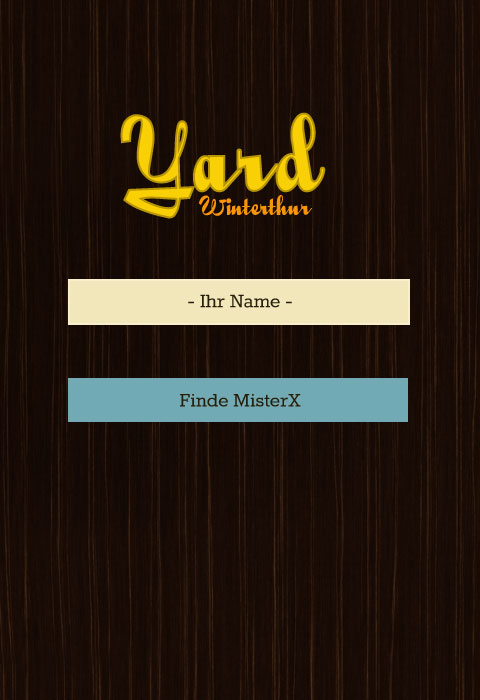
\includegraphics[width=8cm]{Bilder/homeView.jpg}
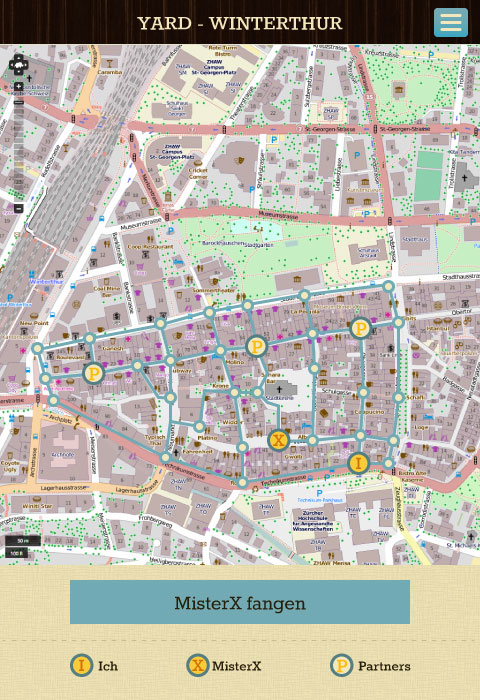
\includegraphics[width=8cm]{Bilder/karteView.jpg}
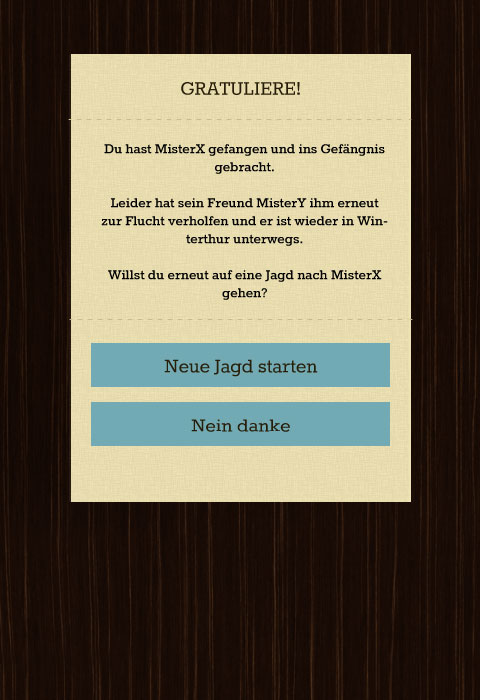
\includegraphics[width=8cm]{Bilder/gefundenView.jpg}
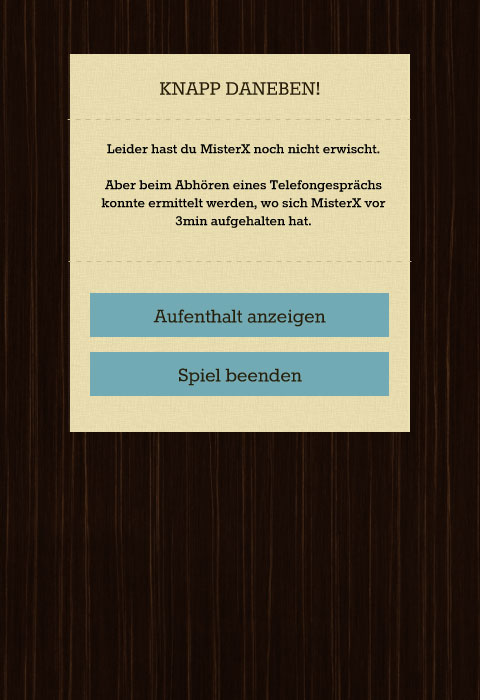
\includegraphics[width=8cm]{Bilder/danebenView.jpg}
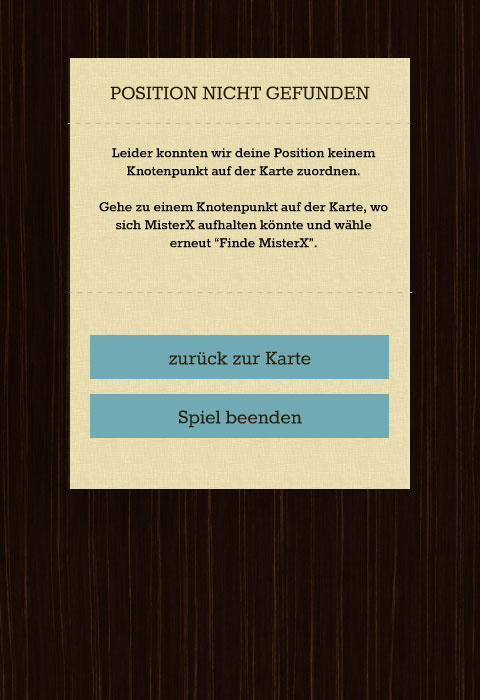
\includegraphics[width=8cm]{Bilder/keinePositionView.jpg}
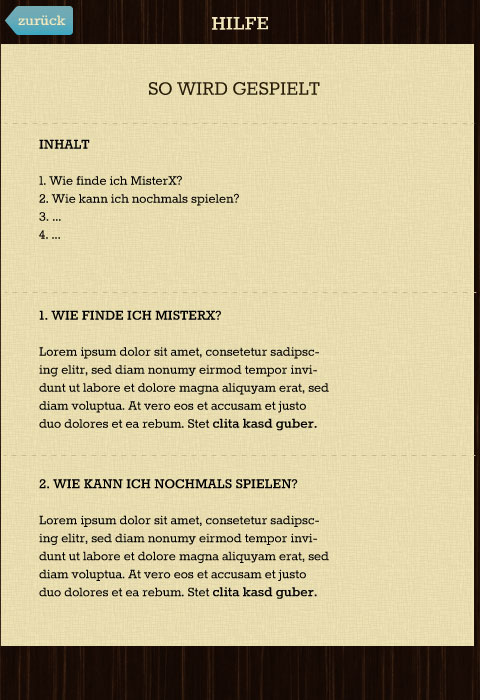
\includegraphics[width=8cm]{Bilder/hilfeView.jpg}
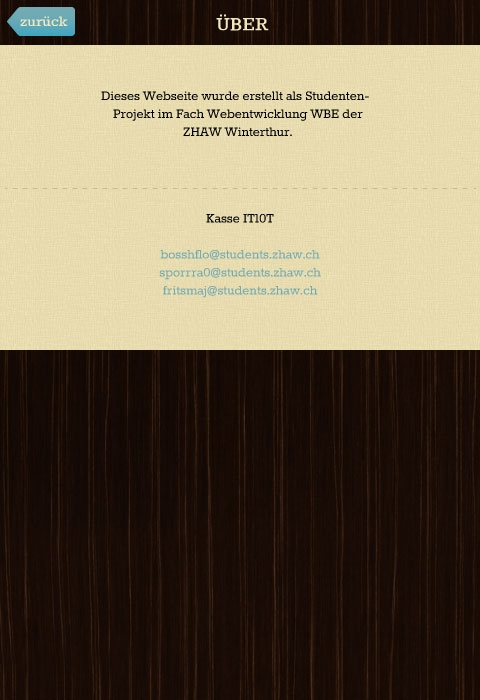
\includegraphics[width=8cm]{Bilder/ueberView.jpg}

\section{Erweiterungsmöglichkeiten}
In diesem Projekt wird eine erste Version des Projektes entwickelt. Es gibt diverse mögliche Erweiterungen, die in einem weiteren Projekt hinzu gefügt werden können. 



\end{document}
